%% Document created 21 March 2021 automatically 
%% from /Users/massimosotgia/Desktop/uni_at_DIFI/Lab_C03/setup.py 

%% Copyright (C) Mattia Sotgia et al. 2021
%% Using class lab_unige.cls
%                                                            
%                                                            
%   **                 **             ******   ****   ****   
%  /**                /**            **////** *///** */// *  
%  /**        ******  /**           **    // /*  */*/    /*  
%  /**       ´´´´´´** /******      /**       /* * /*   ***   
%  /**        ******* /**///**     /**       /**  /*  /// *  
%  /**       **´´´´** /**  /** **  //**    **/*   /* *   /*  
%  /********//********/****** /**   //****** / **** / ****   
%  ////////  //////// /////   //     //////   ////   /´///   
%                                                            
%                                                            
\documentclass[italian, a4paper, 10pt, twocolumn]{../../style/lab_unige}
\usepackage[a4paper, margin=1.75cm, footskip=0.25in]{geometry}

\usepackage[utf8]{inputenc}
\usepackage[T1]{fontenc}

\usepackage[italian]{babel}

% \usepackage{biblatex}

\usepackage[bookmarksopen=true, citebordercolor={0 1 0}, linkbordercolor={1 0 0}, urlbordercolor={0 1 1}]{hyperref}
\usepackage[numbered]{bookmark}

\usepackage{graphicx}
\graphicspath{{../fig/}}
\usepackage{array}
\usepackage{tabulary}
\usepackage{booktabs}

% FOUNDAMENTAL
\usepackage{../../style/custom}

\usepackage{physics}

\usepackage{breqn}
\usepackage{cuted}
\usepackage{txfonts}

\usepackage{lipsum}

%% Define ref types
\newcommand{\reftab}[1]{Tabella {\ref{#1}}}%
\newcommand{\reffig}[1]{Figura {\ref{#1}}}%
\newcommand{\refeqn}[1]{({\ref{#1}})}%
%% PAPER ONLY custom Macros
\newcommand{\Oi}{$O_1$}
\newcommand{\Oii}{$O_2$}
\newcommand{\treSigma}{$3\sigma$}
% \newcommand{\treSigma}{$3\sigma$\space}
\newcommand{\stdNG}[2]{$S_{#1}$($#2$)} %<- ???
\newcommand{\stdErr}[1]{$\varepsilon_{#1}$}
\newcommand{\mstdErr}[1]{\varepsilon_{#1}}
\newcommand{\gLab}{$g_t~=~(~9.8056~\pm~0.0001~\text{ stat}~)~\text{ m/s}^2$}
\newcommand{\ChiSqr}{$\chi^2$\space}
\newcommand{\ChiNdf}{$\chi^2/\text{ndf}$}
\newcommand{\cernroot}{\texttt{root}}
\newcommand{\lr}{$l_{\text{r}}$}
\newcommand{\Ti}[1]{$T_{#1}$}
\newcommand{\Ma}{$M_a$}
\newcommand{\Mb}{$M_b$}
\newcommand{\Tiso}{$T^*$}
\newcommand{\xiso}{$x^*$}
\newcommand{\LrVALUE}{$l_{\text{r}}=(0.800010\pm0.000010)$~m}


%%
\setlength{\columnsep}{6mm}

\begin{document}
    \twocolumn[
    \begin{@twocolumnfalse}
        \title{
            {\raggedright 
\includegraphics[width=0.2\linewidth]{../../style/lab_mark.pdf}\\}
            Misura Sperimentale dell'Accelerazione di Gravità Sfruttando il Pendolo di Kater
        }
        \author{
        Eugenio Dormicchi\textsuperscript{1, 2},
        % Riccardo Pizzimbone\textsuperscript{1}, 
        Giovanni Oliveri\textsuperscript{1},
        Mattia Sotgia\textsuperscript{1}
        }

        \date{
        \textsuperscript{1}Gruppo C03, Esperienza di laboratorio n. 6 \\
        %\textsuperscript{2}In presenza in laboratorio per la presa dati\\
            % Università degli Studi di Genova, Dipartimento di Fisica.\\
            Presa dati-- 
            24 Marzo 2021, 15:00– 18:00; Analisi dati-- 
            30 Marzo 2021
        }
        \maketitle
        
        \begin{abstract}
            \textit{Obiettivo-- }
            Si vuole sfruttare uno strumento di precisione come il pendolo di Kater per ricavare dalla misura accurata del periodo di oscillazione un valore attendibile della misura dell'accelerazione di gravità $g$.
            \textit{Metodi-- }
            Sfruttando il periodo di isocronia \Tiso~ del pendolo di Kater, ricavato dalla posizione $x_b$ della massa mobile \Mb , possiamo ricavare il valore di $g$.
            \textit{Risultati-- }
            Dai valori ottenuti dal fit ricaviamo $g=9.802\pm0.004$ m/s$^2$, che se consideriamo la relazione $\left|g_t-g\right|<3\cdot\sqrt{\mstdErr{g_t}^2+\mstdErr{g}^2} \to 3.6\times10^{-3}\text{ m/s}^2<12\times10^{-3}\text{ m/s}^2$ mostra la compatibilità con il valore teorico \gLab.
            \textit{Conclusione-- }
            L'esperienza mostra come il pendolo reversibile di Kater possa essere utilizzato per effettuare misure fini di $g$, anche se i rapporti \ChiNdf ottenuti dai Fit con \cernroot mostrano dei risultati non perfettamente attendibili.
        
        \end{abstract}
        \vspace{2em}
    \end{@twocolumnfalse}
    ]

    %%%% CORPO DEL TESTO
    %%%% CORPO DEL TESTO

    \section{Obiettivo}
    \label{section:aim}
    Il valore della accelerazione di gravità $g$ può essere ottenuto in diversi metodi, con strumenti via via più precisi, e di conseguenza con risultati che si spera permettano una miglior approssimazione del valore vero di $g$. Il pendolo può essere sfruttato come metodo per misurare tale grandezza, e si è già eseguito l'esperimento sfruttando il pendolo semplice. Per aumentare il livello di precisione dal pendolo semplice si è passati a considerare il pendolo fisico, in particolar modo il pendolo di Kater, che permette di estendere la natura del pendolo "semplice" e anche di eseguire misure con un livello maggiore di dettaglio.\\
    Sfruttando quindi una precisione maggiore e proprietà particolari del pendolo di Kater come pendolo fisico, vogliamo quindi individuare il valore del periodo d'isocronia \Tiso~ caratteristico del pendolo di Kater preso in considerazione e da questo valore ricavare una buona stima di $g$, verificandone infine la compatibilità con il valore noto \gLab.

    \section{Strumentazione}
    \label{section:strument}
    Abbiamo a disposizione i seguenti strumenti:\\
    Calibro ventesimale, di portata 150 mm e sensibilità uguale all'accuratezza dello strumento di 50 $\mu$m;\\
    Calibro da banco di portata 1 m e sensibilità uguale all'accuratezza $10~\mu$m.\\
    Pendolo di Kater (si veda in seguito descrizione dettagliata dell'apparato);\\
    Cronometro elettronico collegato a una fotocellula in grado di misurare una singola oscillazione del pendolo, di portata potenzialmente infinita (molto maggiore comunque dei periodi misurati), e sensibilità 10$^{-7}$ s, che assumiamo anche come accuratezza;\\

    Il pendolo di Kater (\reffig{figure:pendolo}) è costituito da un'asta graduata, dotata di due coltelli sospensione, con una massa fissa a un'estremità (\Ma, massa rossa) e una scorrevole (\Mb, massa blu), posizionata arbitrariamente, vincolata da una vite che la può bloccare all'asta in ben definite posizioni, che sono indicate da $N=25$ fori equidistanti 25~mm tra loro, eseguiti con strumentazione abbastanza precisa da poter trascurare l'incertezza associata a questa distanza. Il pendolo è poi poggiato su un sostegno tramite due perni che si incastrano perfettamente in una sede su una piastra posta orizzontalmente munita di livella a bolla, mantenuta in perfetto equilibrio. Il tutto viene montato su un dispositivo di sostegno in modo che l'asta risulti verticale. Lo strumento è realizzato in maniera tale che i centri di massa delle varie parti costituenti siano allineati su di una retta, intersecante gli assi definiti dai coltelli.\\
    Il pendolo di Kater viene anche definito pendolo reversibile, in quanto possiamo agganciare il pendolo sia sul coltello di sospensione posto sull'estremo vicino alla massa \Ma, che su uno identico posto sull'estremo della massa \Mb, consentendo quindi di misurare due periodi diversi \Ti{1} e \Ti{2}. 

    \begin{figure}[h!]
        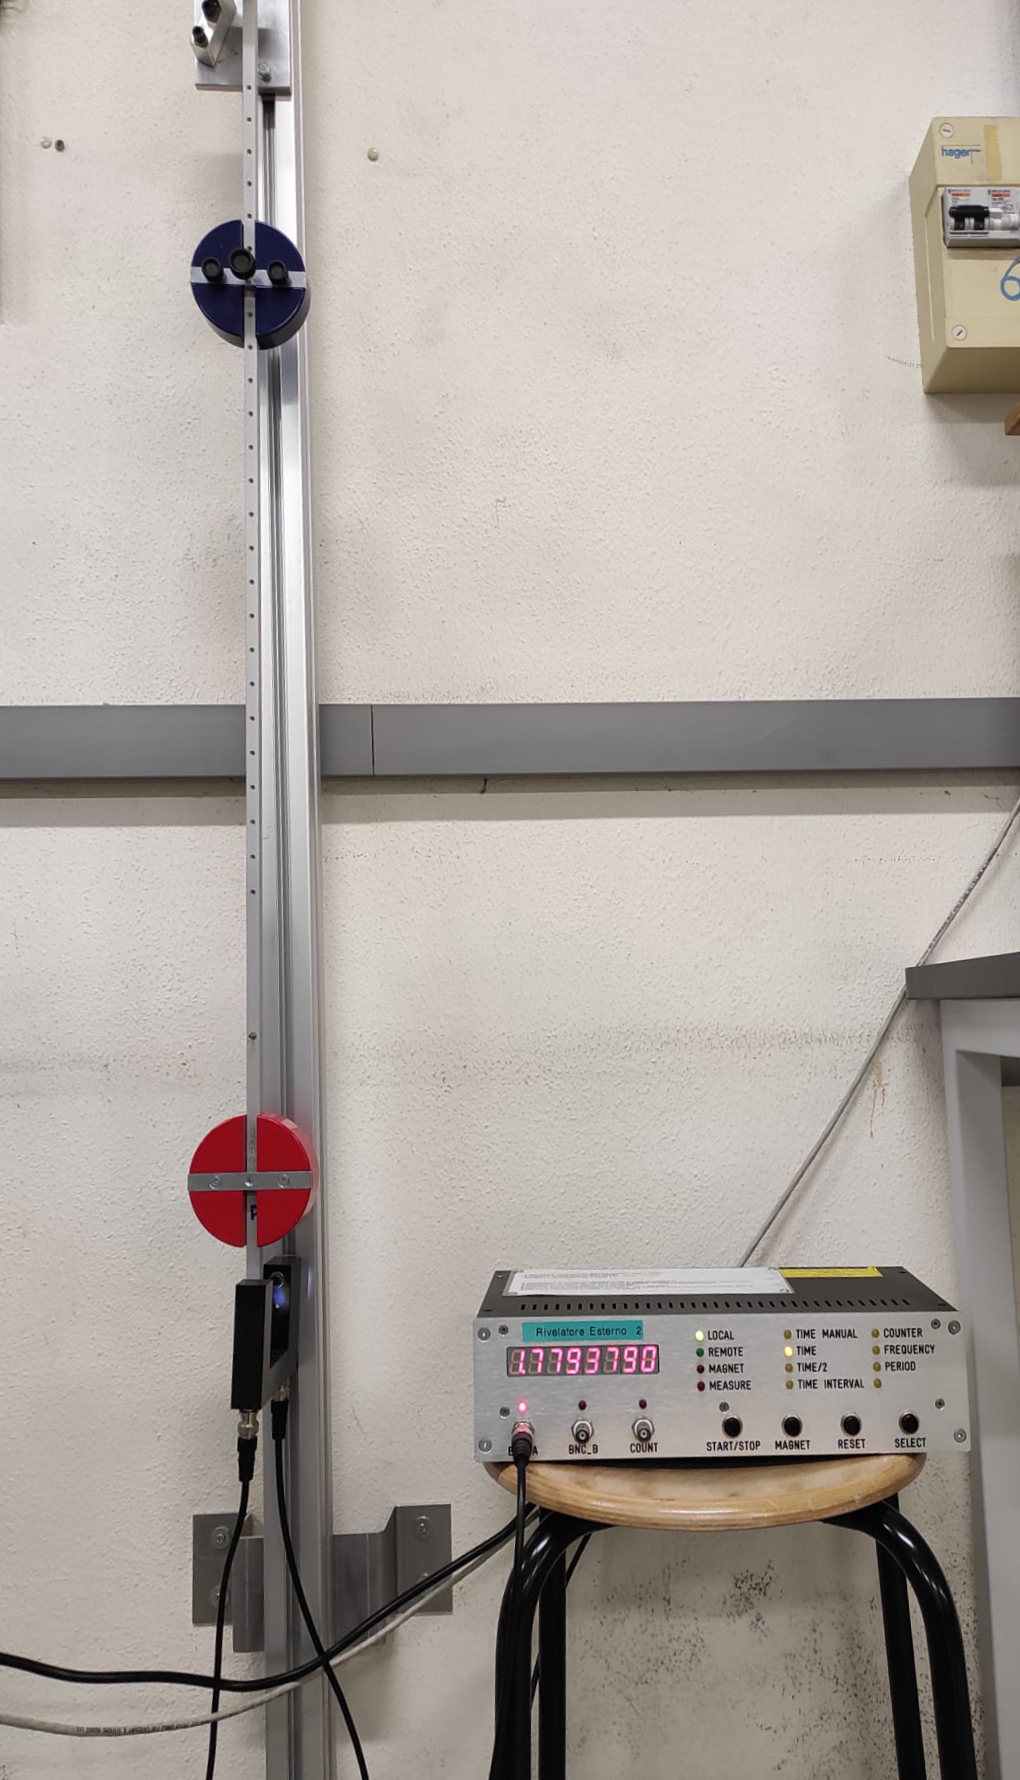
\includegraphics[width=\linewidth]{pendolo.pdf}
        \caption{Fotografia del pendolo di Kater utilizzato. Si mettono in evidenza i punti \Oi~ e \Oii dove sono i due coltelli su cui si può fa oscillare il pendolo; le masse \Ma~(massa rossa) e \Mb~(massa blu). Sono indicate le lunghezze \lr e $L_0$.}
        \label{figure:pendolo}
    \end{figure}

    \section{Metodi}
    \label{section:methods}
    Tutte le misure sono riportate nelle unità del Sistema Internazionale (SI/MKS, ovvero metri, chilogrammi, secondi)
    
    %% MAGARI AGGIUNGERE COMMENTO SU QUANTE CIFRE SI CONSIDERANO E COME APPROSSIMIAMO I VALORI %%
    I valori riportati sono stati approssimati tenendo conto di alcune convenzioni prese. Si approssima l'errore a una cifra significativa se tale cifra è $\geqslant3$, altrimenti se tale cifra è 1 o 2 allora si considerano due cifre significative. Considerando quindi le posizioni decimali significative dell'errore si approssima per eccesso il valore numerico della grandezza.\\

    Si fa spesso riferimento anche alla regola del \treSigma, con la quale si vuole intendere la volontà di trasformare un errore di tipo massimo in errore statistico, ovvero calcolando $\mstdErr{x}~=~\Delta x/\sqrt{3}$.\\% e quindi considerando il valore vero con una probabilità statistica del \treSigma~$\approx99.73\$ di probabilità del dato vero.\\

    Dopo aver eseguito un prima misura del periodo del pendolo considerandolo come pendolo semplice, consideriamo questa volta il pendolo fisico, ovvero come corpo più complesso e dotato di massa.\\
    Il periodo dell’ oscillazione di un pendolo fisico dipende in genere dal momento d'inerzia $I$ rispetto l’asse di sospensione, dal valore di $g$ e dall’ampiezza massima delle oscillazioni. Tuttavia l’esperimento è effettuato nel limite delle piccole oscillazioni per cui la dipendenza dall’ampiezza è trascurabile (isocronia delle piccole oscillazioni).\\
    È possibile quindi valutare $g$ a  partire dalla misura del periodo $T$ e di $I$.  Questo nella pratica non avviene data la difficoltà del calcolo di $I$,

    Il pendolo reversibile, come quello di Kater, elimina questa difficoltà riducendo la misura di $g$ a quella di una serie di lunghezze e intervalli di tempo.\\
    Le misure del periodo di oscillazione vengono effettuate utilizzando alternativamente i due coltelli di sospensione, al variare della posizione sull'asta della massa scorrevole.\\
    L’equazione del periodo (nel limite delle piccole oscillazioni) di un pendolo fisico è $T = 2\pi\sqrt{I/mgh}$, che nel caso del pendolo semplice si può verificare essere $T = 2\pi\sqrt{l/g}$.\\
    Il confronto con il pendolo semplice permette d'introdurre per il pendolo di Kater una grandezza caratteristica: la lunghezza ridotta \lr.
    Definiamo lunghezza ridotta (\lr), la lunghezza del pendolo semplice isocrono a esso \lr~$=~I/mh$. \\
    Misuriamo con un calibro da banco di portata 1~m e sensibilità 10~$\mu$m il valore di \LrVALUE.\\ 
    Attraverso considerazioni di meccanica si ottiene che \lr~$=~h_1+h_2$ con $h_1$ la distanza del coltello di sospensione(\Oi) al centro di massa (CM) e $h_2$ la distanza del coltello di sospensione \Oii~ dal CM.\\
    I risultati ottenuti danno un'indicazione di come deve essere progettata una misura di $g$ tramite un pendolo reversibile.
    Il pendolo deve essere costruito in maniera tale che il suo momento d'inerzia e la posizione del suo centro di massa rispetto agli assi di rotazione, possano essere variate con continuità: ciò viene realizzato utilizzando la massa mobile tra i due coltelli che definiscono gli assi di sospensione.
    In tale modo, con opportuni aggiustamenti della massa mobile, i due assi (fissi) di rotazione possono essere resi isocroni.\\
    Raggiunta una configurazione con assi isocroni, la distanza tra questi ultimi è pari alla lunghezza ridotta del pendolo e quindi è possibile risalire al valore di $g$ tramite una misura di periodo $g=4\pi^2\sqrt{l_{\text{r}}/{T*}^2}$.

    La massa mobile viene spostata partendo dal penultimo foro fino a quello adiacente, distante 25 mm, per un totale di sei posizioni.

    Durante la messa  in moto del pendolo, è necessario aver cura di non introdurre forze perpendicolari al piano d’ oscillazione, in quanto questo comporterebbe oscillazioni anche sul piano normale a quello oscillatorio, introducendo un errore sistematico sulle misure.

    La posizione della massa $x_b$ si può ricavare dalla formula $x_b~=~L_0~+~N~\cdot~25$~mm , dove $L_0$ è la distanza dall’ estremo della sbarra al primo foro successivo alla massa fissa.\\
    $L_0$ è stata misurata, in millimetri, attraverso tre misure distinte mediante l’ uso del calibro. \\
    Otteniamo che $L_0~=~L_{0,~1}~+~L_{0,~2}~+~\text{diametro}_{Mb}/2~= (0.10415)~+~(0.14930)~+~[(0.09040)/2]$~m $ = 0.29865$~m.\\
    Per questa misura introduciamo come errore l'errore ottenuto dalla propagazione degli errori di misura, quindi $50~\mu\text{m}+50~\mu\text{m}+(50/2)~\mu\text{m}=125~\mu\text{m}$, considerando che nel limite in cui effettuiamo un fit non-lineare tramite il metodo dei minimi quadrati, assumiamo di avere errore $\Delta x_b$ trascurabile. Otteniamo quindi una misura staticizzata di $\Delta x_b \to \mstdErr{x_b} = \Delta x_b / \sqrt{3}$.

    Le misure dei periodi \Ti{1} e \Ti{2} sono effettuate con un cronometro digitale azionato dalla fotocellula facendo attenzione a rimanere nel limite di piccole oscillazione e che il fascio di luce venga attraversato da entrambi i lati.
    Poiché il cronometro usato è uno strumento molto sensibile, i periodi ottenuti sono misure non ripetibili;  le misure dei periodi sono perciò effettuate in modo statistico svolgendo 10 misure per ciascun periodo (\Ti{1}, \Ti{2}) per una singola posizione della massa mobile.\\
    I dati raccolti sono riportati in \reftab{table:raw_data}.

    \section{Analisi dati}
    \label{section:analysis}

    \subsection{Trattazione statistica di T}
    I valori di \Ti{1} e \Ti{2} son stati raccolti con 10 ripetizioni per ogni posizione di \Mb~ in modo tale da poter minimizzare le fluttuazione statistiche legate ai valori di $T$. Ricaviamo quindi i valori di $\bar{T_1}=\sum_{i=1}^{10}(T_{1_{(i\times1)}})/10$, con i relativi errori standard $\varepsilon_{T1}=S_{10_i}/\sqrt{10}$. Ripetiamo lo stesso calcolo per tutti i sei valori raccolti di $T_1$ e $T_2$. Riportiamo i valori in \reftab{table:t1_values} e \reftab{table:t2_values}.
    
    \subsection{Rappresentazione e analisi dei dati}
    Riportiamo su un grafico i valori di $T_1$ e $T_2$ sulle ordinate e i valori di $x_b$ sulle ascisse. Osserviamo un andamento parabolico per entrambe le distribuzioni, ben più evidente per la distribuzione dei Periodi di $T_2$, ma si può anche osservare sul grafico dei Periodi $T_1$. 
    Procediamo a costruire due funzioni polinomiali del tipo $y=a_0+a_1\cdot x+a_2\cdot x^2$ che possano essere utilizzate per eseguire un fit non-lineare dei punti dei grafici.

    Dal fit non-lineare ricaviamo il valore di $a_0$, $a_1$ e $a_2$ per i punti di $T_1$ e i valori di $a_0'$, $a_1'$ e $a_2'$ per i punti di $T_2$.
    Considerando quindi la funzione $y=a_0+a_1x+a_2\cdot x^2$ e $y'=a_0'+a_1'\cdot x+a_2'\cdot x^2$ la condizione di isocronia è ottenuta quando $y-y'=0$, ovvero possiamo ricavare $(a_0-a_0')+(a_1-a_1')\cdot x+(a_2-a_2')\cdot x^2=0$ che diventa $A_0+A_1\cdot x + A_2 \cdot x^2$. Quindi ricaviamo il valore di \xiso come
    \begin{equation}\label{eqn:xiso}
        x^* = \frac{-A_1\pm\sqrt{A_1^2-4 A_0 A_2}}{2A_0}=0.837743\text{ m}
    \end{equation}

    Otteniamo due risultati, dei quali teniamo in considerazione solo quella il cui valore è incluso nell'intervallo delle $x$ misurate.
    Sostituendo in $y$ o $y'$ il valore di \xiso otteniamo il valore \Tiso$=1.7951$~s.

    Per calcolare l'errore relativo a \Tiso~ consideriamo i punti le quali ascisse sono più vicine al valore \xiso; ne consideriamo quindi gli errori \stdErr{T1} e \stdErr{T2}, e calcoliamo \[\mstdErr{T*}=\sqrt{\mstdErr{T1}^2+\mstdErr{T2}^2}=0.0004\text{ s}\]

    Per ricavare il valore di $g\pm\mstdErr{g}$ consideriamo la formula
    \[
        g=4\pi^2\frac{l_{\text{r}}}{{T^*}^2}=9.802\text{ m/s}^2
    \]
    con relativo errore
    \[
        \mstdErr{g}=\sqrt{
            \left(
                -\frac{8\cdot l_{\text{r}}\cdot\pi^2}{{T^*}^3}
            \right)^2\cdot\mstdErr{T*}^2+
            \left(
                \frac{4\cdot\pi^2}{{T^*}^2}
            \right)^2\cdot\mstdErr{l_{\text{r}}}^2
        }=0.004\text{ m/s}^2
    \]

    \subsection{Implementazione tramite {\normalfont \cernroot}}
    I Fit e i calcoli successivi sono sati eseguiti con il programma \verb|kater_plot.C| scritto in \verb|C++| sfruttando \cernroot. I dati di input sono raccolti nei file \verb|valori_T1_x.txt| per i periodi $T_1$ e \verb|valori_T2_x.txt| per i periodi di $T_2$, nel formato \verb|xb T1/2 err_xb err_T1/2|.

    Per risolvere l'equazione \ref{eqn:xiso} abbiamo utilizzato la funzione \verb|isocrono_x()| che prende in argomento quattro array che contengono i valori dei parametri (e anche gli errori) restituiti dagli oggetti  \verb|f1| e \verb|f2| della classe \verb|TF1| utilizzate per eseguire il fit non-lineare, dove la funzione \verb|pol2| rappresenta la polinomiale di 2° grado utilizzata.\\
    Il risultato della funzione \verb|isocrono_x()| viene dato come argomento poi alla funzione \verb|get_isoX()|, che presi entrambi i valori dell'equazione, restituisce il valore che corrisponde alla intersezione che possiamo osservare nel grafico.\\
    Dal valore di \xiso si è ricavato \Tiso tramite il metodo \verb|Eval()| della classe \verb|TF1|, che dato il valore di $x$, calcola il valore della funzione in tale punto.

    Per calcolare il valore dell'errore di \Tiso \stdErr{T*} utilizziamo la funzione \verb|get_err_T()|, che individua la coppia di punti più vicina a \xiso e ne calcola l'errore come già trattato.

    Infine le funzioni \verb|get_g()| e \verb|get_gerr()| ricavano il valore di $g\pm\mstdErr{g}$.

    \begin{figure}
        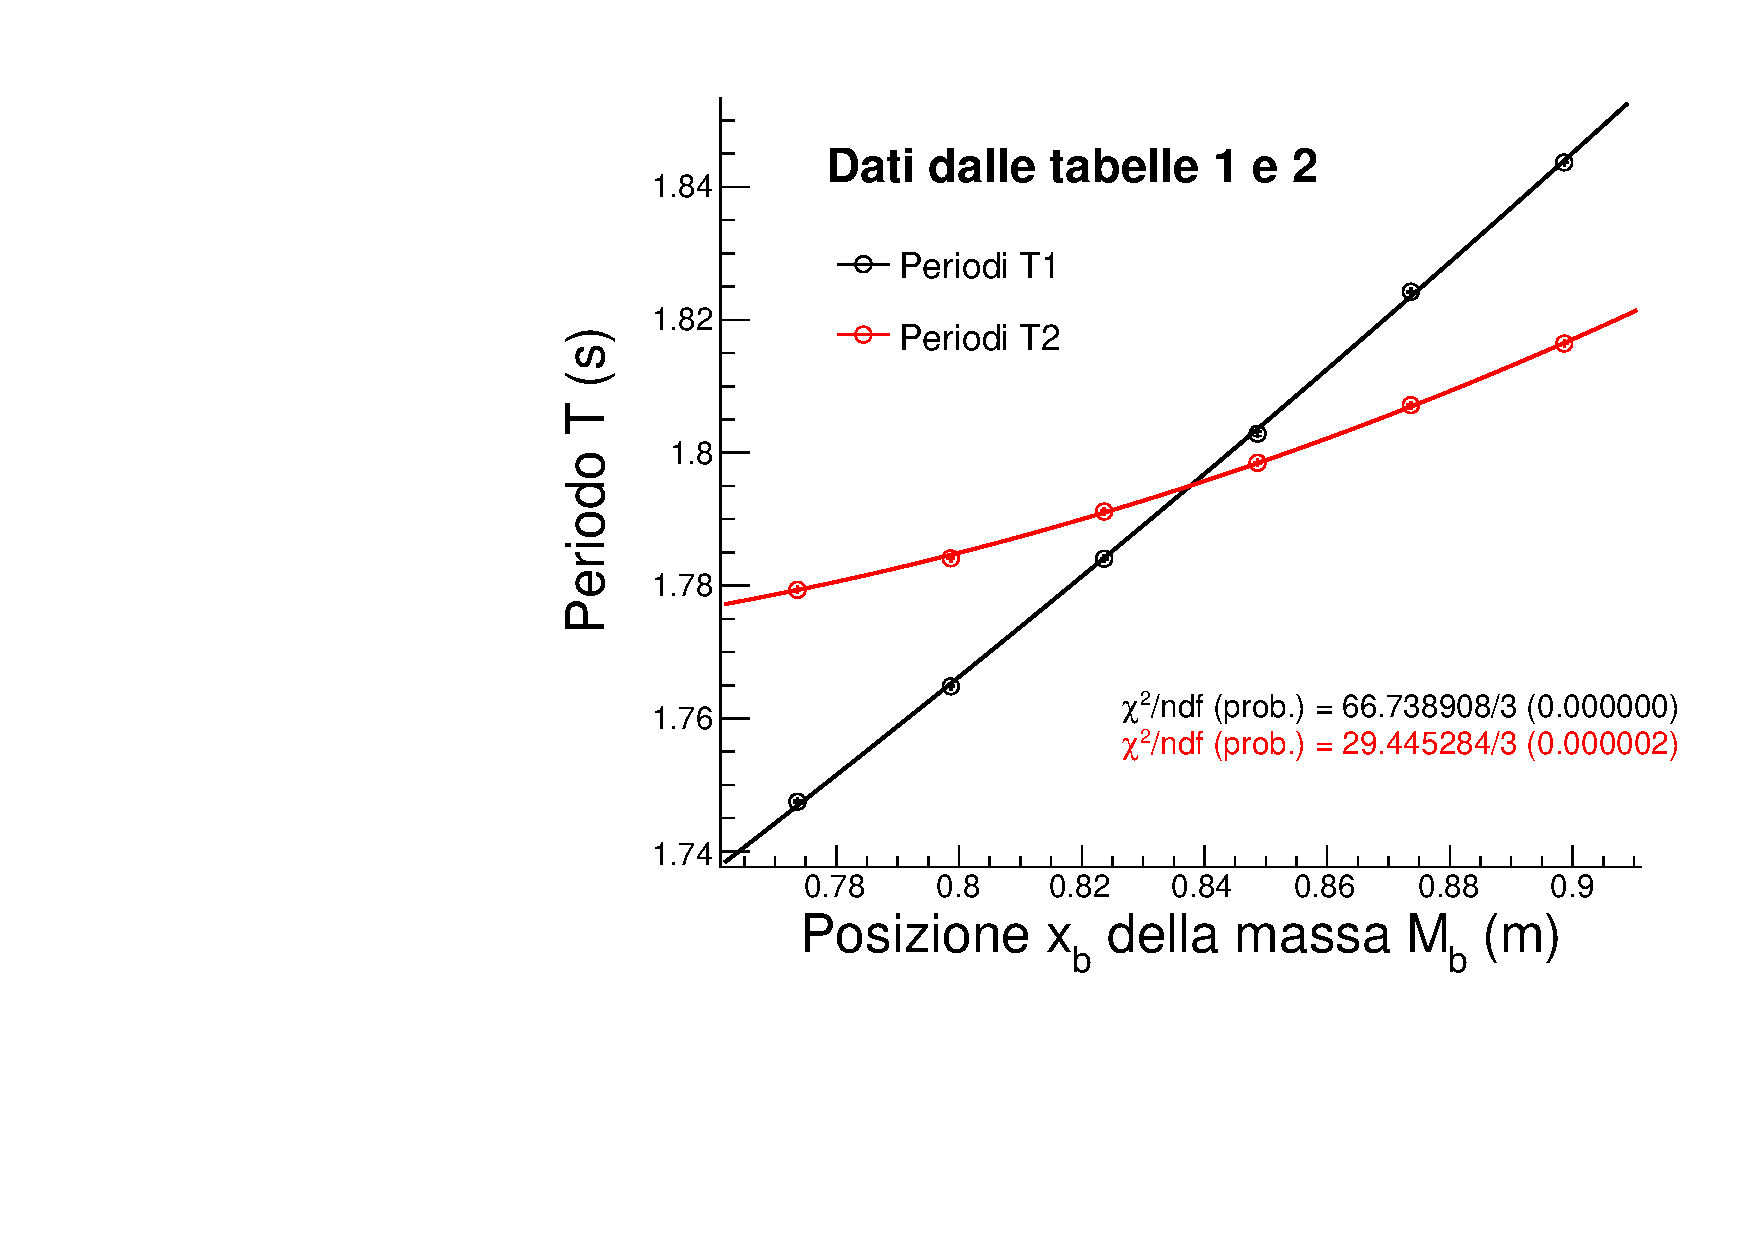
\includegraphics[width=\linewidth]{kater_plot.pdf}
        \caption{Grafico generato con \cernroot. Sono rappresentati i valori di $T_1$ e $T_2$ rispetto a $x_b$, dai dati raccolti in \autoref{table:t1_values} e \autoref{table:t2_values}. Possiamo osservare che il rapporto \ChiNdf è per entrambi i fit piuttosto alto. Questo potrebbe essere legato agli errori che sono molto piccoli sia per i periodi che per le lunghezze. }
        \label{figure:plot}
    \end{figure}

    \begin{table}[t!]
    \centering
    \footnotesize
    \caption{Valori di $x_b\pm\mstdErr{x_b}$ e di $T_1\pm\mstdErr{T1}$ calcolati a partire dai valori presenti in \reftab{table:raw_data} e trattati in \autoref{section:analysis}, sono rappresentati in \reffig{figure:plot} dai punti neri.}
    \label{table:t1_values}
    \begin{tabular}{lcc}
        \hline\hline\\[-1.5ex]
          & Posizione                 & Periodi                  \\[+0.5ex]
          & $x_b\pm\mstdErr{x_b}$ (m) & $T_1\pm\mstdErr{T1}$ (s) \\[+0.5ex] \hline \\[-1.5ex]
        1 & $0.89865\pm0.00007$       & $1.84369\pm0.00009$      \\[+0.5ex]
        2 & $0.87365\pm0.00007$       & $1.82423\pm0.00011$      \\[+0.5ex]
        3 & $0.84865\pm0.00007$       & $1.80286\pm0.00034$      \\[+0.5ex]
        4 & $0.82365\pm0.00007$       & $1.78405\pm0.00011$      \\[+0.5ex]
        5 & $0.79865\pm0.00007$       & $1.76483\pm0.00012$      \\[+0.5ex]
        6 & $0.77365\pm0.00007$       & $1.74748\pm0.00017$      \\[+0.5ex] \hline \\[-1.5ex]
    \end{tabular}
\end{table}

\begin{table}[t!]
    \centering
    \footnotesize
    \caption{Valori di $x_b\pm\mstdErr{x_b}$ e di $T_2\pm\mstdErr{T2}$ calcolati a partire dai valori presenti in \reftab{table:raw_data} e trattati in \autoref{section:analysis}, sono rappresentati in \reffig{figure:plot} dai punti rossi.}
    \label{table:t2_values}
    \begin{tabular}{lcc}
        \hline\hline\\[-1.5ex]
          & Posizione                 & Periodi                  \\[+0.5ex]
          & $x_b\pm\mstdErr{x_b}$ (m) & $T_2\pm\mstdErr{T2}$ (s) \\[+0.5ex] \hline \\[-1.5ex]
        1 & $0.89865\pm0.00007$       & $1.81643\pm0.00008$      \\[+0.5ex]
        2 & $0.87365\pm0.00007$       & $1.80715\pm0.00012$      \\[+0.5ex]
        3 & $0.84865\pm0.00007$       & $1.79848\pm0.00009$      \\[+0.5ex]
        4 & $0.82365\pm0.00007$       & $1.79115\pm0.00011$      \\[+0.5ex]
        5 & $0.79865\pm0.00007$       & $1.78410\pm0.00011$      \\[+0.5ex]
        6 & $0.77365\pm0.00007$       & $1.77936\pm0.00003$      \\[+0.5ex] \hline \\[-1.5ex]
    \end{tabular}
\end{table}

    \section{Risultati}
    \label{section:results}
    Dall'analisi dati in \autoref{section:analysis} abbiamo ottenuto il valore di $g=9.802\pm0.004$ m/s$^2$. Verifichiamo ora tramite la relazione 
    \[
        \left|g_t-g\right|<3\cdot\sqrt{\mstdErr{g_t}^2+\mstdErr{g}^2} \to
    \]
    \[
        \left|9.8056-9.802\right|\text{ m/s}^2<3\cdot\sqrt{(0.0001)^2+(0.004)^2}\text{ m/s}^2 \to
    \]
    \[
        3.6\times10^{-3}\text{ m/s}^2<12\times10^{-3}\text{ m/s}^2
    \]
    che mostra la compatibilità del valore ottenuto con il valore di \gLab~ teorico.
    
    \section{Conclusione}
    \label{section:conclusion}

    \subsection{Controlli}
    Abbiamo ottenuto dall'esperienza un valore di $g$ più preciso e più sensibile rispetto a quello ricavato durante l'esperienza sullo studio del pendolo semplice, dimostrando l'efficacia del pendolo di Kater.\\
    Tuttavia avendo ottenuto un valore del rapporto \ChiNdf~ molto alto (66.7389/3 per $T_1$, 29.4453/3 per $T_2$), e di conseguenza una probabilità del \ChiSqr~ molto bassa ($2.1\times10^{-14}$ per $T_1$ e $1.8\times10^{-6}$ per $T_2$) non potremmo essere fiduciosi delle misurazioni effettuate.

    \subsection{Possibili errori sistematici}
    Possiamo provare a posteriori a individuare alcuni possibili errori sistematici che possono essere intervenuti nelle misurazioni.\\
    Un possibile errore può essere causato dalla forza di attrito viscoso dell’aria, in grado di dissipare energia rallentando il sistema oscillatorio, e diminuendo conseguentemente il valore del periodo misurato. Si è comunque osservato che il pendolo anche dopo diversi minuti il pendolo continuava a oscillare con lo stesso periodo. 
    Un altro possibile errore può essere causato dalla spinta idrostatica dell’aria nei confronti del sistema in grado d'introdurre delle oscillazioni perpendicolari al piano di moto del pendolo, a causa dell'asimmetricità del sistema. Di nuovo si è però stati molto attenti a non introdurre oscillazioni perpendicolari. 
    Infine possiamo considerare l'angolo di oscillazione nel limite delle piccole oscillazioni, in quanto lo spostamento orizzontale $\delta$ abbiamo misurato essere $\approx 0,02$ m, ovvero sottendere un angolo ottenuto come $\phi_0=\arctan{(\delta/L_{\text{totale}})}$, dove consideriamo $L_{\text{totale}}\approx1$ m, ovvero $\phi_0=0.02\text{ rad}\approx1°$.
    \newpage

    \appendix

    \setcounter{table}{0}
    \renewcommand{\thetable}{A\arabic{table}}
    %% this file is for all the tables that go in the appendix as additional data
\begin{table*}[t!]
    \centering
    \caption{Dati grezzi dei periodi \Ti{1} e \Ti{2} misurati alle diverse lunghezze $x_b$.}
    \footnotesize
    \label{table:raw_data}
    \begin{tabular}{l*{6}{c}}
        \hline\hline\\[-1.5ex]
%                              & p1        & p2                 & p3                 & p4        & p5        & p6    
%       dati prima di approx = & 0.89865   & 0.8736499999999999 & 0.8486499999999999 & 0.82365   & 0.79865   & 0.77365
                               & \multicolumn{6}{c}{Misure di $x_b$ calcolate (m)}                                                        \\[+0.5ex] 
                               & \multicolumn{6}{c}{$x_b=\left[L_{0,~1} + L_{0,~2} + \frac{d}{2} + (N_{\text{fori}}\cdot0.025)\right]$ m (errore massimo $\pm1\times10^{-3}$ m)} 
                               \\[+0.5ex] \hline \\[-1.5ex]
        $x_b$                  & 0.899     & 0.874              & 0.849              & 0.824     & 0.799     & 0.774                      \\[+0.5ex] \hline \\[-1.5ex]
                               & \multicolumn{6}{c}{Periodi $T_1$ presi 10 volte per ogni $i$-esimo valore di $x_b$ (s)}                               \\[+0.5ex]
                               & \multicolumn{6}{c}{$T_{1_{(n \times 1)}}, \ldots, T_{1_{(n \times 6)}}$ (errore massimo $\pm10^{-7}$ s)} \\[+0.5ex] \hline \\[-1.5ex]
        $T_{1_{(1 \times i)}}$ & 1.8433475 & 1.8241344          & 1.8010792          & 1.7842967 & 1.7646188 & 1.7469742                  \\[+0.5ex]
        $T_{1_{(2 \times i)}}$ & 1.8438321 & 1.8250191          & 1.8014794          & 1.7831672 & 1.7654354 & 1.7470051                  \\[+0.5ex]
        $T_{1_{(3 \times i)}}$ & 1.8436974 & 1.8243224          & 1.8021671          & 1.7844837 & 1.7653484 & 1.7474456                  \\[+0.5ex]
        $T_{1_{(4 \times i)}}$ & 1.8441519 & 1.8246017          & 1.8026592          & 1.7838530 & 1.7646805 & 1.7473891                  \\[+0.5ex]
        $T_{1_{(5 \times i)}}$ & 1.8438134 & 1.8238088          & 1.8024890          & 1.7842300 & 1.7648372 & 1.7476352                  \\[+0.5ex]
        $T_{1_{(6 \times i)}}$ & 1.8440039 & 1.8240085          & 1.8030486          & 1.7839835 & 1.7650848 & 1.7468288                  \\[+0.5ex]
        $T_{1_{(7 \times i)}}$ & 1.8434289 & 1.8238919          & 1.8031204          & 1.7841418 & 1.7649879 & 1.7475854                  \\[+0.5ex]
        $T_{1_{(8 \times i)}}$ & 1.8437870 & 1.8239454          & 1.8048308          & 1.7838625 & 1.7647196 & 1.7475552                  \\[+0.5ex]
        $T_{1_{(9 \times i)}}$ & 1.8432011 & 1.8243763          & 1.8040768          & 1.7843554 & 1.7644894 & 1.7489131                  \\[+0.5ex]
        $T_{1_{(10\times i)}}$ & 1.8436028 & 1.8242312          & 1.8036150          & 1.7840838 & 1.7641298 & 1.7474017                  \\[+0.5ex] \hline \\[-1.5ex]
                               & \multicolumn{6}{c}{Periodi $T_2$ presi 10 volte per ogni $i$-esimo valore di $x_b$ (s)}                               \\[+0.5ex]
                               & \multicolumn{6}{c}{$T_{2_{(n \times 1)}}, \ldots, T_{2_{(n \times 6)}}$ (errore massimo $\pm10^{-7}$ s)} \\[+0.5ex] \hline \\[-1.5ex]
        $T_{2_{(1 \times i)}}$ & 1.8162160 & 1.8069800          & 1.7978242          & 1.7904099 & 1.7837065 & 1.7793795                  \\[+0.5ex]
        $T_{2_{(2 \times i)}}$ & 1.8162461 & 1.8074008          & 1.7982385          & 1.7919054 & 1.7839124 & 1.7790879                  \\[+0.5ex]
        $T_{2_{(3 \times i)}}$ & 1.8164208 & 1.8066094          & 1.7983828          & 1.7912305 & 1.7838475 & 1.7794034                  \\[+0.5ex]
        $T_{2_{(4 \times i)}}$ & 1.8162922 & 1.8068046          & 1.7984080          & 1.7911800 & 1.7840367 & 1.7794454                  \\[+0.5ex]
        $T_{2_{(5 \times i)}}$ & 1.8165907 & 1.8073671          & 1.7984383          & 1.7912973 & 1.7837570 & 1.7793693                  \\[+0.5ex]
        $T_{2_{(6 \times i)}}$ & 1.8161985 & 1.8071854          & 1.7986348          & 1.7911650 & 1.7840481 & 1.7794584                  \\[+0.5ex]
        $T_{2_{(7 \times i)}}$ & 1.8163087 & 1.8080697          & 1.7989685          & 1.7908471 & 1.7845240 & 1.7793767                  \\[+0.5ex]
        $T_{2_{(8 \times i)}}$ & 1.8162481 & 1.8068933          & 1.7985901          & 1.7912831 & 1.7840374 & 1.7792549                  \\[+0.5ex]
        $T_{2_{(9 \times i)}}$ & 1.8167033 & 1.8072342          & 1.7986484          & 1.7910748 & 1.7848659 & 1.7794661                  \\[+0.5ex]
        $T_{2_{(10\times i)}}$ & 1.8170554 & 1.8069937          & 1.7986683          & 1.7911061 & 1.7842935 & 1.7793790                  \\[+0.5ex]
        \hline
    \end{tabular}
\end{table*}


    \section{Dati estesi}
    Di seguito il listato di output dal programma \verb|kater_plot.C| in \cernroot~(viene utilizzata la versione \verb|6.22/06|).
    {\fontsize{7}{7}
\begin{verbatim}
**********
   PROCESSING G1...
**********

FCN=66.7389 FROM MINOS     STATUS=SUCCESSFUL    490 CALLS        1623 TOTAL
                    EDM=2.00447e-07    STRATEGY= 1      ERROR MATRIX ACCURATE 
 EXT PARAMETER                                   STEP         FIRST   
 NO.   NAME      VALUE            ERROR          SIZE      DERIVATIVE 
  1  p0           1.43416e+00   2.44915e-03   3.73245e-05   5.24168e+00
  2  p1           8.34825e-02   5.56173e-03  -4.48136e-05   4.47109e+00
  3  p2           4.14566e-01   3.31706e-03   3.31706e-03  -1.36586e-01

** CHI2 / NDF ( PROB. ) 66.7389 / 3 ( 2.12974e-14 )


**********
   PROCESSING G2...
**********

FCN=29.4453 FROM MINOS     STATUS=SUCCESSFUL    320 CALLS        1126 TOTAL
                    EDM=2.4987e-09    STRATEGY= 1      ERROR MATRIX ACCURATE 
 EXT PARAMETER                                   STEP         FIRST   
 NO.   NAME      VALUE            ERROR          SIZE      DERIVATIVE 
  1  p0           2.14657e+00   2.02257e-03   2.78818e-06  -1.59149e-01
  2  p1          -1.13945e+00   4.85001e-03  -3.16833e-06  -1.26467e-01
  3  p2           8.59254e-01   2.94517e-03   2.94517e-03  -1.20685e+00

** CHI2 / NDF ( PROB. ) 29.4453 / 3 ( 1.80529e-06 )


**********
   RESULTS ...
**********

x* = 0.837743 +/- 0.0224793
T* = 1.79505 +/- 0.000355199

**********
   COMPATIBLE VALUES
**********

g = 9.80176 +/- 0.00387929
\end{verbatim}}

    Infine in \reftab{table:raw_data} possiamo trovare i valori raccolti in laboratorio prima di essere analizzati.
    
\end{document}
